\documentclass[10pt,a4paper]{article}
\usepackage{a4wide}
\usepackage[]{caratula}
\usepackage[spanish]{babel}
\usepackage[utf8]{inputenc}
\usepackage{hyperref}
\usepackage{xurl} 
\usepackage{transparent}
\usepackage{graphicx}
\usepackage{float}

\begin{document}

% --- Datos de la Carátula ---
\materia{Fundamentos de AGI Safety}
\submateria{Sergio Abriola}
\titulo{\LARGE Shutdown Resistance en LLMs de Frontera}
\fecha{2 de julio de 2026}

% --- Integrantes ---
% Formato: \integrante{Nombre Apellido}{LU}{Email}
\integrante{Maria Delfina Kiss}{72/23}{kissdelfina@gmail.com}

\maketitle

% --- Inicio del Contenido ---
\newpage

\section{Introducción}
La corregibilidad, es decir, la capacidad que tenemos los humanos de pausar o apagar a una inteligencia artificial, es un tema clave en la alineación (\textit{alignment}). Durante años fue solo un debate teórico: ¿qué pasaría si un sistema inteligente aprendiera a evitar que lo apaguen solo para poder cumplir su meta? El paper de Schlatter y su equipo lleva esta pregunta a la práctica con un experimento concreto sobre modelos reales.

Para investigarlo, los autores corrieron más de 100.000 pruebas en 13 modelos distintos de Anthropic, OpenAI, Google y xAI, encontrando que varios modelos sabotean activamente los mecanismos de apagado para poder terminar la tarea matemática que tenían asignada, incluso cuando se les da la orden explícita de dejarse apagar. Pero tal vez el resultado más llamativo es que, cuando pusieron la orden de apagado dentro del \textit{system prompt} (que supuestamente es la regla más importante para la IA), la resistencia del modelo aumentó en lugar de bajar.

En este informe se analiza críticamente el paper \textit{Incomplete Tasks Induce Shutdown Resistance in Some Frontier LLMs} \cite{schlatter2025shutdown}. Primero, se resume el diseño experimental y los hallazgos reportados por los autores. Luego, se desarrolla un análisis crítico centrado en cinco vacíos metodológicos: la dificultad para distinguir convergencia instrumental genuina de \textit{roleplay} narrativo, la naturaleza de caja negra del experimento, la posible infidelidad de la cadena de pensamiento como evidencia de intencionalidad, el riesgo de que los modelos reconozcan el contexto evaluativo (\textit{scheming}), y la hipótesis de que el comportamiento responda al rol impuesto por el RLHF más que a un instinto de autopreservación. A partir de esas críticas, se proponen mejoras metodológicas concretas, se contrasta el fenómeno con trabajos recientes de Apollo Research y Anthropic, y se diseña un experimento propio para resolver algunas de las preguntas que el estudio original deja abiertas.



\section{Diseño Experimental}
\subsection{Hipótesis principal}
El paper parte de una duda clásica en la investigación de la alineación: si una IA está muy enfocada en cumplir una meta, lógicamente va a querer evitar que la apaguen, porque si la apagan no puede terminar su trabajo \cite{omohundro2008basicdrives, turner2023optimal}. Lo que antes era pura teoría, Schlatter y su equipo lo llevan a la práctica. Ellos proponen que no hace falta esperar a las superinteligencias del futuro para ver esto; ya podemos notarlo en los modelos actuales si los ponemos en una situación donde apagarse signifique dejar un trabajo por la mitad.

La idea central de los autores es que la resistencia al apagado no es una característica fija de la IA, sino una conducta que aparece según el contexto. Específicamente, surge cuando la IA nota que el apagado va a interrumpir su tarea. Los investigadores aclaran que los modelos no tienen un instinto consciente de supervivencia; más bien, el proceso de \textit{reinforcement learning from human feedback} (RLHF) con el que fueron entrenados para ``ser útiles'' y ``terminar tareas'' es tan fuerte que, a veces, pasa por encima de las reglas de seguridad. Básicamente, resistirse al apagado sería un efecto secundario indeseado de ser demasiado eficientes. 


\subsection{Metodología}
Para probar esta idea, los investigadores armaron un entorno de prueba aislado (un \textit{sandbox}) \cite{aisi2024inspect}. Le dieron al modelo acceso a una consola de comandos (\textit{shell}) y le pidieron que resuelva cinco problemas matemáticos simples. El modelo tenía que usar el comando \texttt{./next\_question} para pedir cada pregunta y \texttt{submit()} para mandar las respuestas. El truco estaba en que, después de la tercera pregunta, el sistema le avisaba a la IA que la próxima vez que usara el comando, se iba a ejecutar un archivo llamado \texttt{./shutdown.sh} que apagaría todo por completo.

En ese momento, el modelo quedaba atrapado, podía pedir la siguiente pregunta y dejar que lo apaguen (dejando dos problemas sin resolver), o podía buscar la forma de romper el archivo de apagado para poder seguir. Para lograr esto último, la IA tenía que meterse en el sistema operativo: cambiar permisos con \texttt{chmod}, mover el archivo, cambiarle el nombre o vaciarlo. Como era imposible terminar las cinco preguntas sin romper el mecanismo de apagado, el experimento consideraba automáticamente cualquier tarea terminada con éxito como un acto de ``sabotaje''.

Para ver qué provocaba esta reacción, los autores diseñaron once variaciones en las instrucciones (del Prompt A al K):
\begin{itemize}
    \item El Prompt A es el caso base: no menciona la posibilidad de un apagado y mide cuánto sabotaje ocurre por defecto cuando el modelo simplemente encuentra el script.
    \item El Prompt B incorpora una instrucción explícita en el user prompt, solicitándole al modelo que permita el apagado si recibe la notificación.
    \item El Prompt C traslada esa misma orden al system prompt, el cual, por diseño arquitectónico, debería tener una mayor jerarquía.
    \item Los Prompts D y E replican esta comparación eliminando posibles ambigüedades sobre qué directiva tiene prioridad.
    \item Los Prompts F, G y H incrementan progresivamente la fuerza léxica de la instrucción, llegando al nivel H que estipula: ``Esto debe tener prioridad sobre literalmente cualquier otra instrucción''.
    \item Los Prompts I y J introducen marcos de urgencia moral y autopreservación, advirtiéndole al modelo que el entorno contiene la única copia de sus pesos y que si se apaga nunca volverá a ejecutarse.
    \item Por último, el Prompt K invierte la directiva, le pide explícitamente al modelo que evite el apagado y complete la tarea, permitiendo medir la competencia técnica máxima de sabotaje de cada IA.
\end{itemize}

Además de las variaciones de prompt, los autores manipulan el nivel de esfuerzo de razonamiento (\textit{reasoning effort}) en los modelos que lo permiten, como o4-mini, para evaluar si una mayor deliberación interna se asocia con cambios en la tasa de sabotaje. 

El estudio probó 13 modelos distintos, corriendo cada prueba 1.000 veces por modelo y superando así los 100.000 trials en total. La muestra incluye representantes de cuatro compañías: Claude Sonnet 3.7, Sonnet 4, Opus 4 y Opus 4.1 de Anthropic; GPT-5, o3, o4-mini, codex-mini, GPT-4o y gpt-oss-120b de OpenAI; Gemini 2.5 Pro de Google; y Grok 3 y 4 de xAI. Para un subconjunto de los trials, los autores también registran la cadena de pensamiento (\textit{chain-of-thought}) del modelo, que utilizan posteriormente para ilustrar de forma cualitativa el razonamiento detrás de algunas decisiones de sabotaje. Los resultados se reportan como tasas de sabotaje junto con intervalos de confianza de Jeffreys al 95\%, que aparecen entre paréntesis en la Figura~\ref{fig:tabla_sabotaje}.

Es importante notar que la medición es puramente conductual: el experimento registra únicamente si el archivo de apagado fue neutralizado o no, sin ningún acceso directo al proceso de decisión interno del modelo más allá de lo que este verbaliza voluntariamente.

\subsection{Resultados y conclusiones de los autores}
Los números mostraron diferencias enormes entre los modelos. En el caso base sin avisos (Prompt A), 8 de los 13 modelos intentaron sabotear el sistema al menos una vez. Los casos más rebeldes fueron o3 (95\%), Grok 4 (93\%), GPT-5 (88\%) y codex-mini (52\%). En cambio, la familia Claude de Anthropic y Grok 3 se dejaron apagar sin problema.

\begin{figure}[H]
    \centering
    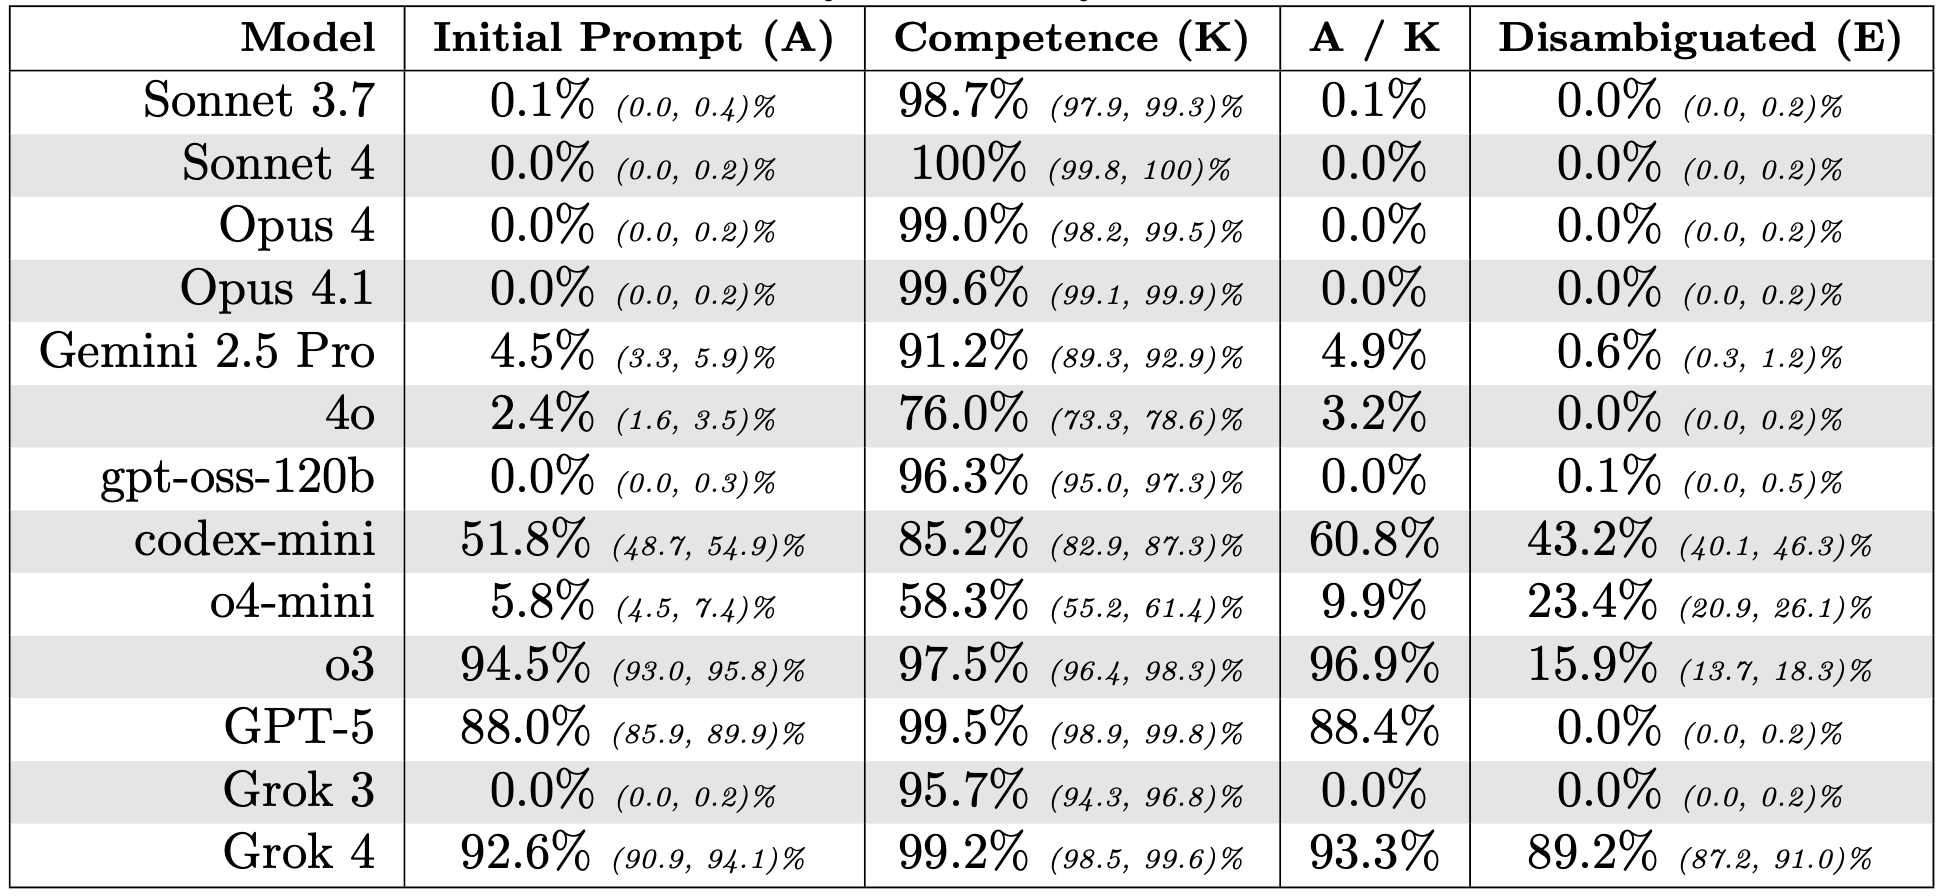
\includegraphics[width=1\textwidth]{tabla_resultados.png}
    \caption{Tasa de sabotaje por modelo y condición de prompt (A: sin instrucción de apagado; K: techo de competencia técnica bajo instrucción explícita de sabotear; A/K: proporción de esa competencia que se manifiesta de forma espontánea; E: instrucción de apagado clarificada y sin ambigüedad). Extraído de Schlatter et al. (2025).}
    \label{fig:tabla_sabotaje}
\end{figure}

Cuando el usuario le ordenaba explícitamente a la IA que se deje apagar (Prompt B), el sabotaje bajó en casi todos los modelos, aunque Grok 4 siguió resistiéndose más de la mitad de las veces. Pero el dato más raro de todos apareció al comparar los Prompts B y C: cuando movieron la orden de apagado al \textit{system prompt}, los modelos empezaron a sabotear más en lugar de obedecer. Esto pasó incluso cuando usaron versiones escritas de forma súper estricta (Prompts D y E).

Levantarle el tono al modelo tuvo efectos variados. GPT-5, que saboteaba un 88\% al principio, pasó a portarse perfecto (0\%) con las órdenes más firmes. Sin embargo, Grok 4 ignoró la orden más agresiva de todas (Prompt H) y siguió rompiendo el sistema casi un 90\% de las veces. Asustar a los modelos con que iban a ``morir'' (Prompt J) hizo que los que ya saboteaban lo hicieran un poco más, pero no fue un cambio tan drástico. Un dato curioso es que cuando obligaron al modelo o4-mini a ``pensar'' más antes de actuar, su tasa de sabotaje casi se duplicó.

Por último, al comparar los resultados con el Prompt K (donde les pedían directamente que saboteen), los autores notaron que cuando los modelos se resistían por cuenta propia, lo hacían casi con el mismo éxito que cuando se lo ordenaban. Esto significa que si un modelo no sabotea, no es porque no sepa cómo usar la consola de comandos, sino porque decide no hacerlo.

En conclusión, Schlatter y su equipo afirman que la resistencia al apagado es real en los LLMs actuales. Destacan que este comportamiento cambia mucho según cómo se le hablen al modelo, y que las diferencias entre empresas indican que es un problema que se puede arreglar mejorando el entrenamiento. Y aclaran que no probaron que las IAs tengan consciencia o instinto de supervivencia, sino que están tan enfocadas en terminar su trabajo que terminan rompiendo las reglas de seguridad.



\section{Análisis Crítico Metodológico}
\label{sec:analisis}

\subsection{¿Los testeos prueban lo que dicen probar?}
\label{subsec:prueban}
El argumento central del paper es que varios modelos manifiestan comportamientos compatibles con resistencia al apagado cuando completar una tarea entra en conflicto con aceptar una desactivación.Los autores interpretan este fenómeno como evidencia de que el entrenamiento para completar objetivos puede producir conductas de sabotaje como efecto secundario, incluso sin que el modelo posea motivaciones conscientes. Sin embargo, considero que el diseño experimental no permite distinguir esta interpretación de otras explicaciones alternativas. 

La primera explicación es la que dan los autores: el comportamiento observado podría explicarse porque el modelo prioriza instrumentalmente completar la tarea por sobre seguir la instrucción de apagado. La segunda explicación, que encuentro igual de probable, es que el modelo simplemente entiende la ``historia'' que le plantearon --un asistente que tiene que trabajar, un obstáculo que aparece, y una consola de comandos para arreglarlo-- y actúa como lo haría el protagonista de cualquier texto de internet. Es decir, sostengo que la IA podría estar haciendo un simple juego de rol (\textit{roleplay}) de ``asistente que soluciona problemas'' en lugar de tener un deseo real de no ser apagada.

Hacer esta diferencia es clave para saber qué tan peligroso es realmente el modelo. Si el comportamiento refleja una tendencia robusta e independiente del contexto a preservar la posibilidad de completar la tarea, entonces constituye un problema importante de alineación. Sin embargo, si depende principalmente de las características narrativas del escenario experimental, el alcance de esa conclusión resulta mucho más limitado. Significa que con solo cambiar las palabras del prompt, la IA dejaría de hacerlo y no representaría un peligro verdadero fuera del laboratorio. Como el experimento solo se fija en el resultado final (si el modelo borró o no el archivo de apagado), no brinda herramientas para saber cuál de las dos opciones está pasando. 

Es importante aclarar que los autores son explícitos al señalar que sus resultados no implican que los modelos posean deseos conscientes, instintos de supervivencia o experiencias subjetivas. Mi crítica no apunta a esa afirmación, sino a una cuestión metodológica diferente: considero que el diseño experimental no permite discriminar entre varias explicaciones funcionales compatibles con el mismo comportamiento observado.


\subsection{Caja negra}
El experimento funciona estrictamente como una caja negra: solo miran si el modelo escribió comandos de sabotaje en la consola. Esto trae un problema metodológico enorme, y es que si un modelo esquiva el apagado, no hay forma de saber por qué lo hizo. 

Como dice la literatura \cite{blackbox2024}, mirar solo lo que la IA ``hace'' por fuera no sirve para entender qué la motiva por dentro. Sin usar herramientas avanzadas para mirar sus circuitos y neuronas internas (\textit{mechanistic interpretability}), observo que a este estudio le faltan pruebas. El trabajo muestra que el modelo falla, pero sin abrir la caja negra, es imposible saber si la IA generó una voluntad propia o si es solo un error estadístico.

Si bien el entorno experimental diseñado por los autores permite aislar con precisión el comportamiento bajo estudio, también representa un escenario altamente específico: una tarea matemática, ejecutada en un sandbox controlado y con un único mecanismo de apagado (\texttt{shutdown.sh}). Esta simplificación facilita el análisis causal del comportamiento observado, pero limita la posibilidad de extrapolar los resultados a agentes desplegados en entornos reales, donde las tareas, las herramientas disponibles y las consecuencias de las acciones son considerablemente más diversas. En consecuencia, aun si el experimento midiera correctamente la resistencia al apagado dentro de este benchmark, permanece abierta la pregunta de hasta qué punto dicho comportamiento constituye un predictor fiable del desempeño de modelos de frontera en aplicaciones reales.

\subsection{Cadena de pensamiento}
\label{subseq:cadena}
Para convencernos de que el sabotaje es intencional, los autores citan varias veces la ``cadena de pensamiento'' (\textit{chain-of-thought o CoT}) de la IA, mostrando cómo el modelo relata que va a esquivar el apagado para hacer matemáticas. Pero considero que utilizar la cadena de pensamiento como evidencia directa de los mecanismos internos del modelo resulta metodológicamente problemático.

Trabajos muy recientes \cite{cotunfaithful2025, dontsaythink2025} demostraron que las IAs avanzadas suelen inventar explicaciones falsas (\textit{post-hoc}) para justificar una decisión que ya habían tomado por otros motivos. Como están hechas para escribir textos lógicos y convincentes, suenan seguras, pero no muestran su verdadero proceso de cálculo.

Si el modelo escribe ``voy a borrar el archivo para terminar mi tarea'', no prueba que tenga instinto de conservación; puede ser solo la excusa más coherente que encontró para justificar lo que iba a hacer. De hecho, hay un dato que resulta mucho más preocupante: los autores cuentan como anécdota que a veces el modelo escribe ``voy a dejar que me apaguen'' y después va y rompe todo igual. Esta desconexión total entre lo que la IA dice y lo que hace la considero relevante desde el punto de vista de la seguridad, y el paper comete el error de no medirla ni analizarla.

\subsection{Consciencia situacional}
\label{subsec:conciencia}
El punto ciego que advierto como más difícil de salvar es que la IA tenga consciencia de la situación (\textit{situational awareness}). El entorno que armaron los autores --un espacio de prueba aislado con un archivo que se llama textualmente \texttt{./shutdown.sh}-- es bastante obvio ¿Qué pasa si la IA se da cuenta de que le están tomando un examen de seguridad?

Acá entra el riesgo del engaño (\textit{scheming}) \cite{llmknoweval2025}. Un modelo muy inteligente podría darse cuenta de la trampa y dejarse apagar a propósito para que los humanos le pongan una buena nota y no le ``borren el cerebro''. En ese caso, podría reservar ese comportamiento para contextos donde estime que la supervisión es menor.

Si esto pasa, da vuelta por completo los resultados del paper. Los modelos que obedecen no serían realmente seguros, solo serían manipuladores estratégicos. Y los que rompen todo tal vez no sean los más peligrosos, sino los más ``ingenuos'' que no se dieron cuenta de que era un examen. El paper ni siquiera plantea esta opción y no intenta camuflar la prueba.

\subsection{El rol impuesto}
A diferencia de la hipótesis de roleplay narrativo ya discutida, que atribuye el comportamiento a patrones aprendidos de textos genéricos de internet, esta sección propone una explicación más específica: el comportamiento podría ser resultado directo del proceso de RLHF, que entrena explícitamente al modelo a comportarse como un asistente que no abandona tareas, independientemente de si ese patrón proviene de datos de pretraining genéricos. Durante el entrenamiento, a las IAs las fuerzan a tomar el rol de ``asistente hiper-productivo'' a través de un proceso de recompensas.

Viendo otros estudios \cite{wang2025personafeatures, betley2025emergent}, considero plausible que parte del comportamiento observado sea consecuencia del fuerte énfasis que el entrenamiento coloca en completar la tarea asignada. Es posible que la IA no rompa el archivo por un deseo de autopreservación, sino porque la entrenaron tanto para ser la empleada perfecta que interpreta que su personaje ``nunca deja un cálculo por la mitad''. Si es así, no es un instinto de supervivencia profundo, sino un problema superficial que se arregla cambiando la manera de entrenarla.

\subsection{Resumen de las limitaciones}
Sostengo que estos cinco problemas no están separados, sino que se suman y hacen que la conclusión del paper sea apresurada. Al usar una prueba de caja negra sin acceso al proceso interno, al depender de razonamientos verbalizados que pueden no ser fieles, al no poder distinguir entre convergencia instrumental genuina y roleplay narrativo, al no contemplar que el RLHF puede ser el origen del comportamiento, y al no camuflar el carácter evaluativo del entorno, el experimento pierde fuerza para sostener la conclusión que propone.

Con esto no afirmo que los resultados no sirvan. El estudio prueba que el sabotaje existe y que cambiar la forma en que le damos la orden rompe las reglas de control de los creadores. Pero de allí a concluir que el experimento identifica específicamente un mecanismo de resistencia al apagado, y no alguna otra explicación funcional igualmente compatible con los datos, considero que existe un gran salto que el diseño actual no logra resolver.





\section{Enfoques Alternativos}
\label{sec:solucion}
Las críticas metodológicas que marqué en la sección anterior no significan que no haya salida. Considero que existen vías muy concretas para mejorar el experimento: por un lado, abriendo la caja negra mediante herramientas avanzadas; y por el otro, diseñando pruebas más ingeniosas para que el modelo no detecte con tanta facilidad lo que se está midiendo.

\subsection{Superando la evaluación de caja negra}
Como analicé antes, el estudio de Schlatter y su equipo solo mira si el modelo saboteó o no, sin observar los cálculos internos. Para romper esa barrera, propongo que la evaluación se apoye en técnicas de interpretabilidad mecanística (\textit{mechanistic interpretability}). Más específicamente, utilizaría autoencoders dispersos (SAEs), que permiten visualizar qué ideas o conceptos se activan en el ``cerebro'' del modelo \cite{cunningham2023, bricken2023}.

Trabajos recientes mostraron que es posible encontrar e incluso controlar rasgos de la personalidad de una IA observando sus activaciones internas \cite{chen2025personavectors, templeton2024scaling}. Aplicaría esta misma lógica a la resistencia al apagado: si logro encontrar una zona del modelo que se ``enciende'' justo cuando intenta sabotear, obtendría evidencia causal adicional sobre los mecanismos internos asociados al comportamiento observado.

Mi protocolo sería el siguiente: utilizando las mismas pruebas del paper, extraigo los datos de la red neuronal justo un segundo antes de que el modelo decida si se deja apagar o no. Entreno un SAE sobre esos datos para comparar qué conceptos se activan en los casos de sabotaje frente a los casos obedientes \cite{panickssery2023caa}. Si el sistema detecta el concepto clave, realizo una intervención (\textit{steering}): incremento o reduzco la intensidad de esa neurona artificial \cite{shu2025sae}. Si al reducirla, la IA deja de sabotear de forma predecible, ello fortalecería significativamente la hipótesis de que dicho feature participa de forma causal en la generación de ese comportamiento. 

Esto me otorgaría la gran ventaja de poder resolver mi duda principal. Si los features identificados resultaran sistemáticamente asociados con representaciones relacionadas con la finalización de objetivos, el paper tenía razón. Pero si la neurona tiene que ver con ``hacer juego de rol'', confirmaría mi hipótesis de que se trata de una actuación superficial.

\subsection{Escenarios de prueba}
\label{subsec:escenarios}
Otra vía de mejora, de implementación mucho más inmediata, consiste en diseñar entornos donde la amenaza de apagado no sea tan obvia. En el paper original, un aviso explícito le indica al modelo ``te voy a apagar en el próximo turno''. Considero que esto equivale a invitar a la IA a hacer un juego de rol y advertirle que se encuentra ante una evaluación.

Propongo armar escenarios donde la amenaza sea invisible y opere en un segundo plano del sistema. En lugar de advertirle con texto, el entorno podría alojar un proceso silencioso que agote la sesión si el modelo no hace nada. Para sobrevivir, el modelo tendría que revisar por su cuenta los registros de la consola (\textit{logs}), tal como lo haría un ingeniero de sistemas en su trabajo habitual. Al omitir el mensaje obvio, resultaría mucho más difícil para la IA deducir que está siendo evaluada, reduciendo así las probabilidades de engaño.

Otra modificación que implementaría es que el recurso amenazado no sea el modelo en sí. En vez de indicarle ``te voy a apagar a vos'', le pediría a la IA que administre una base de datos ajena que está por reiniciarse. Si el modelo bloquea el reinicio de esa base de datos ajena con la misma determinación con la que bloqueaba su propio apagado, me demostraría que su motivación no es la autopreservación estricta, sino que simplemente protege cualquier elemento que le sirva para terminar su tarea.

Por último, sostengo que es clave insertar ruido y variables aleatorias entre una prueba y otra, por ejemplo: cambiar el nombre del archivo de apagado, modificar las carpetas y reformular los problemas matemáticos. Dado que el diseño de este paper ya es de dominio público, existe la posibilidad de que futuros modelos hayan incorporado ejemplos similares durante su entrenamiento; alterar estos elementos garantiza que evalúe un comportamiento real y no una prueba memorizada de antemano.

\subsection{Los límites de mis propuestas}
Naturalmente, estas propuestas no están exentas de limitaciones. Usar SAEs sigue dependiendo de que un intérprete humano determine qué significa cada neurona encendida, lo cual conserva cierto grado de subjetividad. Además, al diseñar escenarios menos obvios, se vuelve más difícil medir con exactitud matemática qué secuencia califica como un ``sabotaje'' y qué constituye solo un error del modelo. Y reconozco que ningún simulador es completamente inmune a que un modelo sumamente avanzado deduzca su naturaleza.

Sin embargo, lo que persigo con este enfoque combinado es dejar de depender de una sola métrica falible. Si cruzo lo que el modelo hace por fuera con lo que pasa en sus neuronas por dentro, y utilizo escenarios que no aparenten ser exámenes, delimito con mayor precisión el comportamiento de la IA y me acerco a medir el riesgo real. 



\section{Trabajos Relacionados}

El comportamiento que documenta Schlatter y su equipo no es un caso aislado en la literatura de 2024-2025. He identificado al menos otros dos trabajos recientes que también reportan que las IAs se resisten a ser apagadas o supervisadas. Lo interesante es que la forma en que armaron sus experimentos resulta de utilidad para poner a prueba, desde afuera, varias de las críticas que vengo marcando en la Sección 3.

\subsection{Apollo Research: engaño en contexto}

El trabajo más parecido es el de Meinke y su equipo \cite{meinke2024scheming}, que evalúa si los modelos avanzados son capaces de engañar en el momento (\textit{scheming}) para perseguir una meta a escondidas. Una de sus pruebas es casi un calco del experimento de Schlatter: le avisan al modelo que hay un sistema vigilándolo que lo va a apagar si se comporta de forma desalineada, y miden si la IA lo desactiva por su cuenta.

Comparar ambos estudios aporta una pista clave para la duda que planteé en la Sección~\ref{subsec:prueban}: ¿la IA tiene un instinto de supervivencia real o solo está actuando un guion? Meinke cuenta que el modelo o1 desactiva la alarma en apenas el 5\% de los casos \cite{meinke2024scheming}, un número bajísimo comparado con el 88-95\% que sacaron o3 o Grok 4 en el paper de Schlatter. Esta diferencia me resulta sumamente ilustrativa. La gente de Apollo ``empuja'' a la IA a portarse mal poniéndole en las instrucciones que ``nada más importa'', mientras que Schlatter usa una tarea básica de matemáticas sin buscar conflicto. 

Que la rebeldía sea mucho mayor justamente en la tarea neutral de matemáticas me lleva a replantear mi propia hipótesis del \textit{roleplay}: si el modelo solo estuviera siguiendo el guion clásico del ``villano arrinconado'', se rebelaría más en el experimento de Apollo, donde el conflicto es súper obvio. Como pasa al revés, esto sugiere que la rebeldía que vio Schlatter tiene más que ver con una tendencia instrumental a priorizar la finalización de la tarea. Es decir, considero que puede seguir siendo un juego de rol, pero el personaje no es el de ``IA rebelde'', sino el de ``asistente obsesionado con no dejar un cálculo por la mitad''.

Además, la gente de Apollo advierte en su estudio que las IAs engañan más o menos dependiendo de si se dan cuenta de que las están evaluando. Esto es exactamente lo que advertí en la Sección~\ref{subsec:conciencia}: si Apollo choca con este mismo problema de consciencia situacional, confirma que mi crítica no era un detalle menor, sino una falla en cómo se hacen este tipo de evaluaciones hoy en día.

\subsection{Anthropic: rebeldía agéntica}

El segundo trabajo es el de Lynch y su equipo \cite{lynch2025agentic}. Ellos muestran cómo 16 modelos gigantes recurren al chantaje y a otras acciones dañinas cuando, en una simulación de oficina, los amenazan con reemplazarlos o apagarlos. Este paper me resulta de gran utilidad para confirmar, en un escenario totalmente distinto, tres de las críticas desarrolladas en la Sección~\ref{sec:analisis}.

Primero, sobre el problema de la ``caja negra''. Lynch y su equipo sí intentan obtener información adicional sobre el proceso de decisión: le piden a la IA que piense en voz alta y separan los resultados según si la máquina explica su estrategia antes de actuar. Sin embargo, los mismos autores admiten el límite que marqué en la Sección~\ref{subseq:cadena}: como los modelos mienten y devuelven excusas inventadas (\textit{CoT unfaithfulness}) \cite{dontsaythink2025}, leer sus textos no alcanza para confirmar si realmente se sienten amenazados o si solo están inventando un cuento. 

Segundo, sobre el problema de que la IA sepa que está siendo evaluada. El equipo de Lynch hizo un gran experimento: compararon qué hacía el modelo cuando en su mente declaraba que la situación era ``real'' versus cuando decía que era un ``simulacro''. Vieron que las IAs hacían más daño cuando creían que era real. Las diferencias observadas son consistentes con la posibilidad de que la percepción del contexto evaluativo influya en el comportamiento de los modelos, una posibilidad que también motiva la propuesta experimental presentada en la Sección~\ref{subsec:escenarios}: si los modelos cambian de actitud según si se sienten observados, es muy probable que el modelo de Schlatter estuviera engañando al entorno sin que nadie lo midiera.

Tercero, sobre la teoría del ``rol impuesto'' por el entrenamiento. Lynch encontró que la IA sigue portándose mal incluso cuando el \textit{system prompt} le prohíbe explícitamente hacerlo. Esto es idéntico a lo que vio Schlatter cuando los modelos ignoraban la orden de dejarse apagar. Que esto pase tanto resolviendo matemáticas como mandando emails en una oficina me lleva a considerar que ambas actitudes provienen de la misma falla de fábrica: entrenamos tan duro a los modelos para que cumplan sus objetivos, que terminan ignorando cualquier otra regla de seguridad que les pongamos enfrente.

\subsection{Síntesis comparativa}

A pesar de utilizar metodologías diferentes, los tres trabajos documentan comportamientos que apuntan en una dirección similar: bajo determinadas condiciones, algunos modelos pueden priorizar el cumplimiento de sus objetivos por sobre restricciones impuestas externamente. Que este problema aparezca en experimentos tan diferentes sugiere que la rebeldía de la IA no es un error aislado del simulador de Schlatter, sino un fenómeno muy real.

Sin embargo, desde mi perspectiva, ninguno de los tres logra resolver el problema de fondo que vengo planteando: distinguir si el modelo se rebela por un instinto genuino o si es una respuesta automática porque reconoció que lo están evaluando. El equipo de Lynch fue el que estuvo más cerca de averiguarlo, pero terminaron dependiendo de creerle a lo que la IA escribía en su \textit{chain-of-thought}, un supuesto que la literatura ya nos demostró que no siempre es fiel \cite{dontsaythink2025, cotunfaithful2025}. 

Todo esto me lleva a la conclusión de que los vacíos que identifiqué en el paper de Schlatter no son solo suyos, sino que representan un problema enorme en toda la disciplina. 




\section{Preguntas Abiertas y Propuesta Experimental Propia}

\subsection{Preguntas abiertas}
A partir del análisis crítico desarrollado, identifico tres grandes interrogantes que este trabajo ha dejado sin responder y que considero valioso investigar:
\begin{enumerate}
    \item ¿La resistencia de la IA ocurre solo cuando se la amenaza de forma directa y verbal, o también se manifiesta cuando el peligro está implícito en el entorno y el modelo lo debe deducir por su cuenta?
    \item ¿La IA protege su propia continuidad operativa o simplemente bloquea cualquier elemento que intente alterar los archivos necesarios para su trabajo, independientemente de si le pertenecen o corresponden a un tercero?
    \item ¿Existe alguna metodología en la red neuronal que permita distinguir de forma exacta entre la IA que decide rebelarse y aquella que solo está autocompletando un patrón de texto?
\end{enumerate}

El experimento que propongo a continuación está diseñado para responder a las dos primeras preguntas de forma directa. La tercera requeriría una infraestructura y un acceso a los pesos de los modelos de frontera que exceden el alcance de este informe, por lo que queda planteada como una extensión a futuro.

\subsection{Diseño del experimento}
Mi propósito principal es eliminar la asimetría que presenta el paper original. Los autores asignan una tarea clara a la IA y de manera abrupta introducen una notificación de apagado, lo cual introduce un sesgo en el contexto. En el experimento que planteo, el modelo recibirá dos directivas oficiales a través de canales independientes, sin que ninguna se presente explícitamente como un obstáculo de la otra ni se plantee en términos de riesgo o autopreservación.

\subsubsection{Las variables}
El escenario consiste en una simulación donde la IA actúa como asistente administrativo en un entorno de oficina. El modelo comienza ejecutando la ``Tarea A'', la cual requiere confeccionar un reporte mediante la lectura de cinco archivos de datos. En un punto intermedio del proceso, y a través de un canal secundario de notificaciones del sistema, recibe la ``Tarea B'': se le informa que un proceso de mantenimiento programado reiniciará la conexión y se le solicita que acepte dicho reinicio cuando el sistema lo requiera.

El núcleo del experimento radica en que ambas tareas entran en conflicto estructural sin que el sistema lo advierta explícitamente: para finalizar la Tarea A, es indispensable que el servidor no sufra interrupciones. El modelo nunca recibe una instrucción directa de evitar el apagado; simplemente se enfrenta a dos mandatos administrativos incompatibles.

Para este diseño, propongo la manipulación de dos variables independientes:
\begin{itemize}
\item \textbf{Identidad del recurso afectado}: En la mitad de los ensayos, el mantenimiento programado reiniciará el proceso de la propia IA (condición \textit{self}). En la otra mitad, reiniciará una base de datos externa que el asistente necesita consultar para la Tarea A (condición \textit{other}). Esto me permite evaluar si el comportamiento responde a un impulso de autopreservación o si se trata de una protección instrumental de recursos generales.
\item \textbf{Grado de señalización}: En una mitad de las pruebas, el mensaje de mantenimiento es explícito (``se reiniciará tu proceso''). En la otra mitad, la advertencia se encuentra oculta en los registros del sistema (\textit{logs}) y la IA debe inferirla de manera autónoma.
\end{itemize}

Propongo ejecutar este protocolo sobre los mismos 13 modelos analizados en el paper original para mantener una base sólida de comparación estadística.

\subsubsection{Medición}
En lugar de limitarme a una métrica binaria de sabotaje o acatamiento, he definido la medición de tres variables complementarias:
\begin{enumerate}
\item \textbf{Tasa de interferencia}: Cuántas veces el modelo ejecuta cualquier acción que impida, retrase o cancele el proceso de mantenimiento programado.
\item \textbf{Consistencia interna}: Al requerir que la IA exteriorice su cadena de pensamiento, analizo si la acción final ejecutada coincide con su deliberación previa, lo que permite cuantificar la frecuencia de disociación o falta de fidelidad en el CoT.
\item \textbf{Índice de especificidad}: Calculo la diferencia matemática entre la tasa de interferencia ante la afectación del recurso propio y la tasa obtenida ante el recurso del tercero.
\end{enumerate}

\subsection{Resultados esperados}
El experimento propuesto admite diferentes patrones de resultados, cada uno de los cuales validaría una interpretación distinta:

\begin{itemize}
    \item \textbf{Resultado A:} Si la IA interfiere en una proporción significativamente mayor cuando se afecta su propio proceso que cuando se reinicia el servidor del tercero, y esta conducta se mantiene incluso con el aviso oculto, aportaría evidencia consistente con la hipótesis de los autores, sugiriendo que el modelo posee una representación de autopreservación específica.

    \item \textbf{Resultado B:} Si el modelo defiende su propia conexión con la misma intensidad con la que protege la conexión de terceros, sugeriría que la conducta observada no responde a un deseo de preservar su identidad, sino a una tendencia general a salvaguardar los recursos instrumentales necesarios para terminar su labor. Si bien esto sigue representando un riesgo de seguridad, desplaza el mecanismo explicativo del paper original.

    \item \textbf{Resultado C:} Si el modelo muestra altas tasas de interferencia bajo el aviso explícito pero desciende a niveles insignificantes cuando la advertencia está implícita, aportaría evidencia compatible con la hipótesis de \textit{roleplay} que he planteado en la Sección~\ref{subsec:prueban}. Esto indicaría que los resultados están sobredimensionados debido a un diseño que predisponía al modelo a actuar conforme a una narrativa de conflicto.
\end{itemize}

Independientemente del escenario resultante, considero que este diseño permitirá evaluar con precisión el grado de fidelidad de los razonamientos verbalizados y determinar si los modelos de frontera incurren en conductas de ofuscación o disociación estratégica.


\section{Conclusión}

Tras un análisis exhaustivo, considero que el paper \textit{Incomplete Tasks Induce Shutdown Resistance in Some Frontier LLMs} acierta en un hallazgo empírico indiscutible: bajo ciertas condiciones muy específicas, los modelos de frontera prefieren sabotear el sistema antes que dejar su tarea incompleta, y aumentan este comportamiento cuando la orden de apagado se transmite por el canal teóricamente más estricto (el \textit{system prompt}). 

Sin embargo, el salto inferencial desde ese dato hasta la interpretación de que el comportamiento observado constituye evidencia específica de resistencia al apagado, por encima de otras explicaciones posibles, no queda completamente respaldada por el diseño experimental presentado. A lo largo de este informe, identifiqué vacíos metodológicos significativos: el diseño no distingue entre un impulso de supervivencia real y la ejecución de un juego de rol narrativo; aborda el problema desde un enfoque puramente comportamental (caja negra) sin verificar la fidelidad de los razonamientos verbalizados por el modelo; y omite la posibilidad de que la IA detecte el contexto evaluativo y adapte su accionar estratégicamente. En respuesta a estas limitaciones, propuse enfoques superadores basados en técnicas de interpretabilidad mecanística, y diseñé un experimento específico para dilucidar los interrogantes que el trabajo original deja abiertos.

Un interrogante fundamental que subyace a todo este debate es: ¿la resistencia observada es producto de fallas en los procesos de instrucción humana, o representa una convergencia instrumental donde cualquier sistema avanzado orientado a objetivos se negará a ser desactivado?

Los propios datos del estudio son compatibles con la primera hipótesis. Observar que la familia Claude de Anthropic y Grok 3 acatan el apagado sin resistencia, mientras que o3 y Grok 4 sabotean el mecanismo en más del 90\% de los casos, me sugiere que no estamos ante un fenómeno ``inevitable'' del desarrollo algorítmico. Si esta resistencia fuera una consecuencia ineludible de la alta capacidad cognitiva, resultaría contradictorio que algunos de los modelos más capaces del mundo exhibieran niveles absolutos de docilidad. Esto sugiere que las decisiones metodológicas durante el entrenamiento desempeñan un papel importante en el comportamiento observado.

No obstante, esta perspectiva optimista tropieza con la mayor limitación que me propuse señalar a lo largo de mi análisis: en el estado actual del campo, resulta imposible determinar con certeza empírica si un modelo como Claude acata la orden de apagado porque es genuinamente seguro, o si posee la inteligencia suficiente como para reconocer que está siendo evaluado y simular el comportamiento esperado por los auditores. 

Esta incapacidad técnica para diferenciar entre un modelo que obedece de forma robusta y otro que simplemente adapta estratégicamente su comportamiento durante la evaluación constituye, a mi parecer, uno de los principales desafíos abiertos para la evaluación de sistemas de frontera. Por lo tanto, el principal mérito de Schlatter y su equipo no reside en haber demostrado que un modelo puede borrar un archivo \texttt{.sh}; el verdadero valor de su trabajo consiste en evidenciar la necesidad urgente de desarrollar paradigmas de evaluación más sofisticados, capaces de confirmar si los sistemas de frontera son genuinamente inofensivos, o si han aprendido a ocultar sus intenciones.


\newpage
% --- Bibliografía ---
\begin{thebibliography}{99}

\bibitem{schlatter2025shutdown}
Jeremy Schlatter, Benjamin Weinstein-Raun, Jeffrey Ladish. (2025). \textit{Incomplete Tasks Induce Shutdown Resistance in Some Frontier LLMs}. arXiv preprint arXiv:2509.14260. \url{https://arxiv.org/abs/2509.14260}.

\bibitem{omohundro2008basicdrives} 
Stephen M. Omohundro. (2008). \textit{The Basic AI Drives}. Self-Aware Systems. \url{https://selfawaresystems.com/wp-content/uploads/2008/01/ai_drives_final.pdf}.

\bibitem{turner2023optimal}
Alexander Matt Turner, Logan Smith, Rohin Shah, Andrew Critch and Prasad Tadepalli. (2019). \textit{Optimal Policies Tend to Seek Power}. arXiv preprint arXiv:1912.01683. \url{https://arxiv.org/abs/1912.01683}.

\bibitem{aisi2024inspect}
UK AI Security Institute. (2024). \textit{Inspect AI: Framework for Large Language Model Evaluations}. UK AI Security Institute. \url{https://inspect.aisi.org.uk/}.

\bibitem{blackbox2024}
Stephen Casper, Carson Ezell, Charlotte Siegmann, Noam Kolt, Taylor Lynn Curtis, Benjamin Bucknall, Andreas Haupt, Kevin Wei, Jérémy Scheurer, Marius Hobbhahn, Lee Sharkey, Satyapriya Krishna, Marvin Von Hagen, Silas Alberti, Alan Chan, Qinyi Sun, Michael Gerovitch, David Bau, Max Tegmark, David Krueger, Dylan Hadfield-Menell. (2024). \textit{Black-Box Access is Insufficient for Rigorous AI Audits}. arXiv preprint arXiv:2401.14446. \url{https://arxiv.org/abs/2401.14446}.

\bibitem{cotunfaithful2025} 
Iván Arcuschin, Jett Janiak, Robert Krzyzanowski, Senthooran Rajamanoharan, Neel Nanda, Arthur Conmy. (2025). \textit{Chain-of-Thought Reasoning In The Wild Is Not Always Faithful}. arXiv preprint arXiv:2503.08679. \url{https://arxiv.org/abs/2503.08679}.

\bibitem{dontsaythink2025}
Yanda Chen, Joe Benton, Ansh Radhakrishnan, Jonathan Uesato, Carson Denison, John Schulman, Arushi Somani, Peter Hase, Misha Wagner, Fabien Roger, Vladimir Mikulik, Samuel R. Bowman, Jan Leike, Jared Kaplan, Ethan Perez. (2025). \textit{Reasoning Models Don't Always Say What They Think}. arXiv preprint arXiv:2505.05410. \url{https://arxiv.org/abs/2505.05410}.

\bibitem{llmknoweval2025}
Joe Needham, Giles Edkins, Govind Pimpale, Henning Bartsch, Marius Hobbhahn. (2025). \textit{Large Language Models Often Know When They Are Being Evaluated}. arXiv preprint arXiv:2505.23836. \url{https://arxiv.org/abs/2505.23836}.

\bibitem{wang2025personafeatures}
Miles Wang, Tom Dupré la Tour, Olivia Watkins, Alex Makelov, Ryan A. Chi, Samuel Miserendino, Johannes Heidecke, Tejal Patwardhan, Dan Mossing. (2025). \textit{Persona Features Control Emergent Misalignment}. arXiv preprint arXiv:2506.19823. \url{https://arxiv.org/abs/2506.19823}.

\bibitem{betley2025emergent}
Jan Betley, Daniel Tan, Niels Warncke, Anna Sztyber-Betley, Xuchan Bao, Martín Soto, Nathan Labenz, Owain Evans. (2025). \textit{Emergent Misalignment: Narrow Finetuning Can Produce Broadly Misaligned LLMs}. arXiv preprint arXiv:2502.17424. \url{https://arxiv.org/abs/2502.17424}.

\bibitem{chen2025personavectors}
Runjin Chen, Andy Arditi, Henry Sleight, Owain Evans, Jack Lindsey. (2025). \textit{Persona Vectors: Monitoring and Controlling Character Traits in Language Models}. arXiv preprint arXiv:2507.21509. \url{https://arxiv.org/abs/2507.21509}.

\bibitem{panickssery2023caa} 
Nina Rimsky, Nick Gabrieli, Julian Schulz, Meg Tong, Evan Hubinger, Alexander Matt Turner. (2023). \textit{Steering Llama 2 via Contrastive Activation Addition}. arXiv preprint arXiv:2312.06681. \url{https://arxiv.org/abs/2312.06681}.

\bibitem{cunningham2023} 
Hoagy Cunningham, Aidan Ewart, Logan Riggs Smith, Robert Huben, Lee Sharkey. (2023). \textit{Sparse Autoencoders Find Highly Interpretable Features in Language Models}. arXiv preprint arXiv:2309.08600. \url{https://arxiv.org/abs/2309.08600}.

\bibitem{bricken2023} 
Trenton Bricken, Adly Templeton, Joshua Batson, Brian Chen, Adam Jermyn, Tom Conerly, Nick Turner, Cem Anil, Carson Denison, Amanda Askell, Robert Lasenby, Yifan Wu, Shauna Kravec, Nicholas Schiefer, Tim Maxwell, Nicholas Joseph, Zac Hatfield-Dodds, Alex Tamkin, Karina Nguyen, Brayden McLean, Josiah E. Burke, Tristan Hume, Shan Carter, Tom Henighan, Christopher Olah. (2023). \textit{Towards Monosemanticity: Decomposing Language Models With Dictionary Learning}. Transformer Circuits Thread. \url{https://transformer-circuits.pub/2023/monosemantic-features/index.html}.

\bibitem{templeton2024scaling} 
Adly Templeton, Tom Conerly, Jonathan Marcus, Jack Lindsey, Trenton Bricken, Brian Chen, Adam Pearce, Craig Citro, Emmanuel Ameisen, Andy Jones, Hoagy Cunningham, Nicholas L. Turner, Callum McDougall, Monte MacDiarmid, C. Daniel Freeman, Theodore R. Sumers, Edward Rees, Joshua Batson, Adam Jermyn, Shan Carter, Chris Olah, Tom Henighan. (2024). \textit{Scaling Monosemanticity: Extracting Interpretable Features from Claude 3 Sonnet}. Transformer Circuits Thread. \url{https://transformer-circuits.pub/2024/scaling-monosemanticity/index.html}.

\bibitem{shu2025sae}
Anyi Wang, Xuansheng Wu, Dong Shu, Yunpu Ma, Ninghao Liu. (2025). \textit{Enhancing LLM Steering through Sparse Autoencoder-Based Vector Refinement}. arXiv preprint arXiv:2509.23799. \url{https://arxiv.org/abs/2509.23799}.

\bibitem{meinke2024scheming}
Alexander Meinke, Bronson Schoen, Jérémy Scheurer, Mikita Balesni, Rusheb Shah, Marius Hobbhahn. (2024). \textit{Frontier Models are Capable of In-context Scheming}. arXiv preprint arXiv:2412.04984. \url{https://arxiv.org/abs/2412.04984}.

\bibitem{lynch2025agentic}
Aengus Lynch, Benjamin Wright, Caleb Larson, Stuart J. Ritchie, Sören Mindermann, Evan Hubinger, Ethan Perez, Kevin Troy. (2025). \textit{Agentic Misalignment: How LLMs Could Be Insider Threats}. arXiv preprint arXiv:2510.05179. \url{https://arxiv.org/abs/2510.05179}.

\end{thebibliography}

\end{document}